\section*{Introduction}
\label{sec:introduction}

The increasing demand for efficient urban logistics has led to the exploration of innovative delivery solutions. One such approach is the exploration of drone-based deliveries system. One interesting idea to research in that field is the integration of public transport systems to improve the performance of drone-based systems. Indeed, in many cases, the delivery system would operate alongside regular public transport service, which it could use to reduce the distance drones have to travel. An example could be using a drone to transport the package from the pickup point to a bus station, put the package in a bus, then have another drone pick the package at another bus stop for the last mile delivery to the delivery point. 

\begin{wrapfigure}{r}{0.5\textwidth}
    \centering
    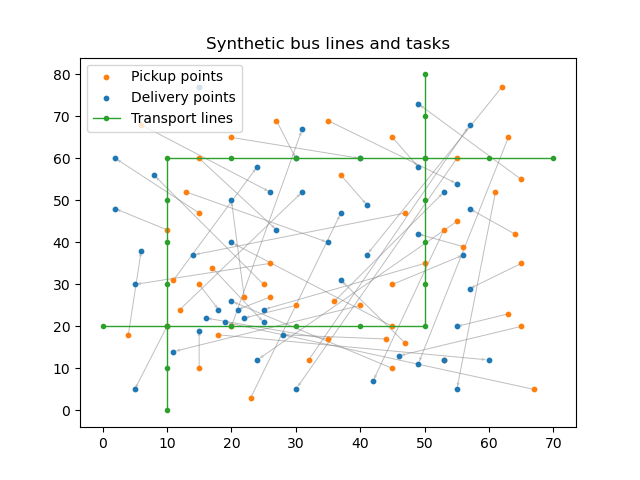
\includegraphics[width=0.5\textwidth]{../fig/synthetic_tasks.png}
    \caption{A synthetic bus network with synthetic drone tasks}
    \label{fig:intro}
\end{wrapfigure}

In researching the pertinence of such a system, one could use synthetic data like randomised tasks and geometric bus lines, an example of which is found in Figure \ref{fig:intro}. Although a good starting point, it is an interesting question to ask ourselves to what extend results obtained with this method correspond to the reality.

The goal of this project is to provide the data that will allow to solve this question, by anchoring the experiment to the real world. Using availlable data about public transport in Switzerland, we export bus lines trajectories as well as timetables. Then, using statistical data about the population density and the location of shops, we generate tasks that match the surronding geography. This will enable a comparison with synthetic data and provide a validation framework for previously developed assumptions. Finally, we implement a basic metrix (total drone distance) to compare the impact a drone-and-bus delivery system could have (i) around a suburban bus route; (ii) in a full agglomeration and (iii) in the synthetic environment shown in Figure \ref{fig:intro}.
